\documentclass{article}
\title{暗号の数学入門 — 素数が鍵になるしくみ}
\author{TeX 図書館}

\begin{document}

\section{読み方 — この本の地図と 3 つの道具}

暗号は「秘密の合言葉」の学問だと思われがちですが、現代暗号の本質は\textbf{計算の難しさを鍵に使う}ことです。掛け算は一瞬、素因数分解は途方もなく時間がかかる。この\textbf{「易しい方向と難しい方向」の差}が、インターネットの安全を支えています。

つまずきの原因は、ほぼ 1 つ。\textbf{「暗号化」と「本人確認」という 2 つの用途を混ぜて理解しようとする}こと。同じ数学(公開鍵暗号)が 2 つの逆向きの使い方をする、という構造を先に押さえれば、RSA も署名も 1 つの仕組みの 2 面に見えてきます。

\subsection{全 10 節の見取り図}

節の配分は次のとおりです。

\begin{enumerate}
\item 第 1 節: 読み方。暗号化・復号・鍵の 3 語を決めます。
\item 第 2 節: 古典暗号。ずらして隠す発想と、その限界。
\item 第 3 節: モジュラ計算。余りで考える算数の道具。
\item 第 4〜5 節: 鍵配布問題と素因数分解。現代暗号の動機と材料。
\item 第 6 節: RSA 暗号。公開鍵と秘密鍵の仕組み。
\item 第 7〜8 節: ハッシュと電子署名。改ざん検出と本人確認。
\item 第 9 節: 応用と限界。TLS、パスワード、量子コンピュータ。
\item 第 10 節: まとめと次の一歩。
\end{enumerate}

各節の終わりには\textbf{解答の指針}を置きます。答えの丸写しではなく、どの計算をどの方向に流すかを書く欄です。まず自力で 5 分考えてから、その欄を開いてください。

\subsection{本書で使う 3 つの言葉}

\begin{itemize}
\item \textbf{暗号化}: 平文(読める文)を、鍵を使って読めない文に変えること。
\item \textbf{復号}: 暗号文を、鍵を使って平文に戻すこと。
\item \textbf{鍵}: 変換の仕方を決める数や情報。秘密にする部分と公開してよい部分がある。
\end{itemize}

\begin{quote}
\textbf{【注意】}\ 暗号の強さは「解読が不可能」という意味ではありません。\textbf{解読に必要な計算量が、現実的な時間で終わらない}という意味です。技術が進めば「現実的」の線は動きます。だから暗号の研究は、難しさの根拠を常に更新する作業です。
\end{quote}

\textbf{解答の指針:}\ 暗号の問題では、まず「誰が何を知っていて、誰が何を知らないか」を 1 行ずつ書く。次に、情報の流れを「平文 → 暗号化 → 通信 → 復号 → 平文」の 4 段で書き、各段で使う鍵が公開鍵か秘密鍵かを明示する。流れ図が描ければ、あとは各段の計算(第 3 節以降の道具)に落とすだけです。

\section{古典暗号 — ずらして隠す}

最も古い発想は\textbf{文字をずらす}ことです。アルファベットを 3 つずらして A を D にする(シーザー暗号)。ずらす幅が鍵で、受取人は同じ幅を逆に戻せば復号できます。

\subsection{頻度分析: 規則性は必ず漏れる}

シーザー暗号の鍵は 25 通りしかないので、全部試せば終わりです。さらに深刻な弱点が\textbf{頻度分析}です。英語では E が最も多く出る、TH や IN が頻出する、という言語の統計的な癖が、暗号文にそのまま写ります。最も多い文字を E と仮定すれば、ずらし幅は 1 通に決まる。

教訓は明快です。\textbf{隠したい情報の統計的な癖が、変換を通しても残る限り、暗号は弱い}。現代暗号の設計目標の 1 つが「暗号文が平文の統計を漏らさない」ことです。置換だけでなく、繰り返しパターンを消す操作(ブロック化、初期ベクトル)が必要になるのはこのためです。

\subsection{鍵が変われば文も変わる: ケルクホフスの原則}

「暗号方式を秘密にすれば安全だ」という考えは 19 世紀に否定されました。\textbf{方式は公開しておき、鍵だけを秘密にする}。これを\textbf{ケルクホフスの原則}と呼びます。方式が漏れるのは時間の問題であり、方式に依存した安全は長持ちしない。公開されて研究されてなお破られない方式だけが、実用に残ります。この原則があるからこそ、この本のように暗号の仕組みを全部説明して安全が成立します。

\begin{quote}
\textbf{【注意】}\ 「独自の暗号を自作すれば安全」という考えは、この原則の逆で、危険の代表例です。自作の方式は専門家の解析を受けていないので、弱点が残ったままです。実務の原則は「検証済みの標準を使い、鍵の管理を固める」です。
\end{quote}

\textbf{解答の指針:}\ 古典暗号の問題では、(1) ずらし幅(鍵)を明示し、(2) 暗号文の文字頻度を数えて言語の癖と比べる、(3) 「統計が漏れる」ことを弱点として書く。自作暗号を評する問題では、ケルクホフスの原則に照らして「方式公開で安全が保てるか」を確認します。頻度表を 1 つ書けるかどうかが、古典暗号の理解の目安です。

\section{モジュラ計算 — 余りで考える時計の算数}

現代暗号の舞台は\textbf{余りの世界}です。13 時は 1 時、60 分は 0 分。時計の針は端まで行くと原点に戻る。\textbf{ある数で割った余りだけを考える算数}をモジュラ計算(合同算術)と呼びます。

\[ 14 \bmod 12 = 2 \]

読み方は「14 を 12 で割った余りは 2」。この世界では足し算・掛け算が普通にできますが、結果はすべて余りに折り返されます。17 + 10 は 27 ですが、12 の世界では 3 です。掛け算も同様で、\( 7 \times 8 = 56 \) は 12 の世界では 8 になります。

\begin{figure}
\centering
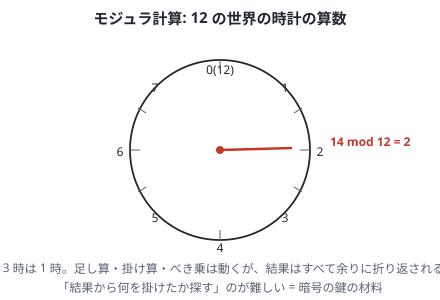
\includegraphics[width=0.85\textwidth]{figures/mod-clock.svg}
\caption{モジュラ計算: 12 の世界では 14 も 2 も同じ場所を指す}
\end{figure}

\subsection{逆算の難しさが鍵になる}

余りの世界の重要な性質は、\textbf{「掛けた結果から、何を掛けたかを推測するのが難しい」}ことです。実数の世界なら 56 を見て「7 と 8」と割り出すのは易しい(56 ÷ 7)。しかし余りの世界では、\( 7 \times 8 \equiv 8 \pmod{12} \) を満たす組が複数あり、結果 8 から答えを一意に復元できません。

さらに重要な道具が\textbf{べき乗}です。\( 3^{5} \bmod 17 \) のような計算は順に掛けて余りを取るだけで易しい。しかし逆に「\( 3^{x} \equiv 13 \pmod{17} \) を満たす \( x \) を求めよ」(離散対数問題)は、素朴には \( x \) を 1 つずつ試すしか方法がなく、数が大きくなると現実的でない。この\textbf{順方向は易しい・逆方向は難しい}という非対称が、次節以降の鍵の材料です。

\begin{quote}
\textbf{【注意】}\ 余りの計算は、途中で余りを取っても最後に取っても同じ結果になります(分配的に動く)。これが実装の基本で、大きなべき乗は「1 回ごとに余りを取る」ことで数字が爆発せずに済みます。暗号の実装では、この小さな工夫が性能の生命線です。
\end{quote}

\textbf{解答の指針:}\ モジュラ計算の問題では、(1) 何で割るか(法)を明示する、(2) 掛け算は途中で余りを取って小さく保つ、(3) 逆問題(どの数を掛けたか、べき乗の指数を求める)は「試すしかない」ことを確認して、難しさの根拠にする。時計のたとえで「13 時は 1 時」を書けるかが、最初の理解の目安です。

\section{鍵配布問題 — 鍵はどう渡すか}

古典暗号の共通の弱点がこれです。\textbf{暗号化と復号に同じ鍵を使う}(共通鍵暗号)場合、鍵を相手に渡す必要があります。しかし鍵を安全に渡す方法があったら、その方法で本文も渡せるのではないか。\textbf{鍵の配布には、鍵の配布が必要}という堂々巡りです。

\subsection{共通鍵の運用と限界}

共通鍵暗号(AES など)自体は今も現役で、速くて強い。問題は配布だけです。歴史的には、事前に別の安全な経路(手渡し、外交バッグ(封印した輸送))で鍵を配る運用で回避してきました。しかしインターネットでは、\textbf{会ったことのない何百万の相手と、その場で安全な通信}を始める必要があります。事前の手渡しは不可能です。

この堂々巡りを破る発想が、1970 年代の\textbf{公開鍵暗号}です。「暗号化に使う鍵は公開してよい、復号の鍵だけ持っていればいい」方式が作れれば、鍵を渡す必要が消えます。

\subsection{非対称性: 2 つの鍵で 1 つの仕組み}

公開鍵暗号では、\textbf{暗号化(誰でもできる)と復号(鍵の持ち主だけができる)に異なる鍵}を使います。電話帳にたとえるのが定番です。誰でも彼の電話番号(公開鍵)を見て電話をかけられる。しかし受話器を取れるのは彼(秘密鍵)だけです。

この一方向性を実現するには、\textbf{順方向が易しく逆方向が難しい数学の構造}が必要です。その材料が、次節の素因数分解です。

\begin{quote}
\textbf{【注意】}\ 「公開鍵で暗号化したものは秘密鍵で復号できる」のと同時に、「秘密鍵で変換したものは公開鍵で確かめられる」も成り立ちます。後者は復号ではなく\textbf{署名}の使い方(第 8 節)です。2 つの鍵の役割を「暗号用 / 確認用」と区別して書くと混乱しません。
\end{quote}

\textbf{解答の指針:}\ 鍵配布の問題では、(1) 誰と誰が、最初に共有していない状態から始まるかを確認する、(2) 共通鍵方式だと「鍵の配布」という同じ問題が再帰的に出ることを書く、(3) 公開鍵方式の解決は「暗号化は公開・復号は秘密」の分離、と表現する。電話帳のたとえを 1 行で書けるかが理解の目安です。

\section{素数と因数分解 — 一方向の扉}

公開鍵暗号の土台は、\textbf{素数}の計算の性質です。素数は 1 と自分でしか割れない数(2, 3, 5, 7, 11, …)。すべての整数は素数の積としてただ 1 通りに書けます(13 = 13、21 = 3 × 7、300 = 2\(^{2}\) × 3 × 5\(^{2}\))。

\subsection{掛け算は易しく、分解は難しい}

2 つの大きな素数(300 桁など)を掛け算するのは、コンピュータにとって一瞬です。しかし積(600 桁)を渡されて\textbf{元の 2 つの素数に分解する}(素因数分解)のは、現在知られている最速の方法でも途方もない時間がかかります。桁数が倍になるごとに、必要な時間は激増します。

これが\textbf{一方向関数}です。「易しい方向」と「難しい方向」がはっきり分かれている計算。掛け算の方向なら何万人分の計算でも一瞬、分解の方向なら世界中のコンピュータを回しても一生かからない。\textbf{この時間の崖が、鍵の代わりになります}。

\subsection{なぜ「ただ 1 通り」が重要か}

素因数分解の一意性(素因数分解の一意分解定理)は、暗号の正しさの保証です。復号の計算が、暗号化の逆になっていることを数学的に示せる。\textbf{鍵がある人は必ず元の文に戻せ、鍵がない人は戻せない}、という保証が「たった 1 通りの分解」から出ます。素数が「何の役に立つのか」という問いへの答えの核心はここにあります。

\begin{quote}
\textbf{【注意】}\ 素因数分解が難しいことは証明されておらず、「現在は速い方法が知られていない」という状態です。暗号の信頼は、数十年にわたる世界中の解析攻撃が失敗し続けているという実績で支えられています。だから標準暗号は、新しい研究成果が出るたびに鍵長を増やして更新されます。
\end{quote}

\textbf{解答の指針:}\ 素因数分解の問題では、(1) 小さい数で「掛け算は易しい・分解は難しい」を実際に確認する(26 = 2 × 13 は易しいが、463 を自分で分解してみる)、(2) 桁数と必要時間の関係(桁が増えると崖のように増える)を書く、(3) 「一方向関数が鍵の代わりになる」を一言で表現する。小さい数での手計算の経験が、600 桁の話を直感に繋げます。

\section{RSA 暗号 — 素数 2 つが作る鍵}

いよいよ仕組み本体です。RSA(開発者の頭文字)は、\textbf{素因数分解の難しさ}を直接使う公開鍵暗号です。仕組みは、実は小学算術の道具(余りの掛け算とべき乗)だけで説明できます。

\subsection{鍵の作り方}

\begin{enumerate}
\item 大きな素数を 2 つ選ぶ: \( p \) と \( q \)(実際は数百桁)。
\item その積 \( N = pq \) を計算する。\textbf{N は公開してよい}(分解は難しいから)。
\item 公開鍵は \( N \) と公開指数 \( e \)、秘密鍵は \( p \) と \( q \) から作る復号用の数 \( d \)。
\end{enumerate}

\textbf{ポイントは、秘密鍵 \( d \) を作るには \( p \) と \( q \) が必要}なことです。公開情報の \( N \) から \( d \) を作るには、\( N \) を素因数分解する必要があります。つまり\textbf{鍵の強度は、素因数分解の難しさそのもの}です。

\subsection{暗号化と復号の流れ}

平文を数 \( m \) とみなして、次の計算で変換します。

\[ c = m^{e} \bmod N \]

これが暗号文です。誰でも(公開鍵を持つ人なら)計算できます。受取人は秘密鍵 \( d \) を使って

\[ m = c^{d} \bmod N \]

を計算すると、元の \( m \) が戻ってきます。なぜ戻るかの証明は、第 3 節の余りの世界の性質(べき乗の周期性)と、\( d \) と \( e \) の作り方の対応で与えられます。\textbf{易しい方向のべき乗(暗号化)を、難しい方向には戻せない(秘密鍵がないと復号できない)}。扉が 1 方向にだけ開く仕組みです。

\begin{figure}
\centering
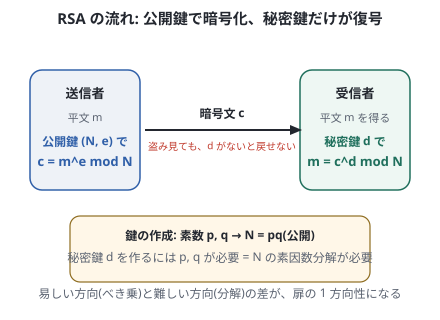
\includegraphics[width=0.9\textwidth]{figures/rsa-flow.svg}
\caption{RSA の流れ: 公開鍵で暗号化、秘密鍵だけが復号}
\end{figure}

\begin{quote}
\textbf{【注意】}\ RSA の安全性は「素因数分解が難しい」ことだけでなく、\textbf{鍵長(素数の大きさ)と運用}に依存します。2048 ビット未満の鍵、使い回しの素数、乱数の質の低さ、といった実装の甘さが、数学の難しさより先に破られます。「数学は安全でも運用は別」というのが実務の鉄則です。
\end{quote}

\textbf{解答の指針:}\ RSA の問題では、(1) 公開されるもの(\( N, e \))と秘密のもの(\( p, q, d \))を 2 欄の表に書き分ける、(2) 暗号化は \( m^{e} \bmod N \)、復号は \( c^{d} \bmod N \) と流れを書く、(3) 秘密鍵を作るには素因数分解が必要、と強度の根拠を明示する。小さい数(例: \( p=3, q=11, N=33 \))で実際に暗号化と復号を回してみると、仕組みが手に届きます。

\section{ハッシュ — もとに戻せない指紋}

暗号と並ぶもう 1 つの柱が\textbf{ハッシュ関数}です。任意の長さのデータを、固定長の短い値(ハッシュ値)に変換します。\textbf{ハッシュは復号できません}。戻る方向が存在しない、というのが特徴です。

\subsection{ハッシュの 3 つの性質}

\begin{itemize}
\item \textbf{同じ入力は必ず同じ値}: データの指紋として使える。
\item \textbf{少しでも変わると全然違う値になる}: 改ざんの検出に使える。
\item \textbf{もとに戻せない(一方向)}: ハッシュ値から元データを復元できない。
\end{itemize}

\begin{figure}
\centering
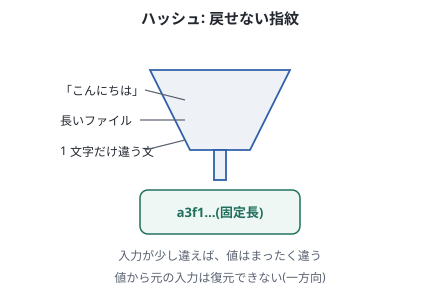
\includegraphics[width=0.9\textwidth]{figures/hash-funnel.svg}
\caption{ハッシュ: どんな入力も固定長の指紋になり、戻せない}
\end{figure}

使い方は幅広い。\textbf{改ざん検出}：ファイルのハッシュ値を配布元が公開し、ダウンロード後に計算して一致を確かめる。1 バイトでも書き換わっていれば値は全く違うものになり、検出できます。\textbf{パスワードの保存}：サービスはパスワード本体ではなくハッシュ値だけを持ち、ログイン時に入力をハッシュして比較します。これなら、データベースが漏れても元のパスワードは出てきません。

\subsection{なぜ「戻せない」ことが安全なのか}

ハッシュ値から元の入力を探すには、\textbf{候補を片っ端から入力して試す}しかありません(総当たり)。この「戻すには総当たりしかない」性質が、パスワード保存に最適です。一方で攻撃者の総当たりも成立するので、実際には\textbf{salt(合言葉の追加)と反復回数}で試すコストを意図的に上げます。簡単なパスワードは、総当たりで数秒で戻される、という現実もこの節の帰結です。

\begin{quote}
\textbf{【注意】}\ 「暗号化」と「ハッシュ」は別物です。暗号化は\textbf{鍵で戻せる}、ハッシュは\textbf{戻せない}。パスワードを「暗号化して保存」するのは誤りで(鍵が漏れると全部戻される)、正しくは「ハッシュして保存」です。この 2 語を区別して使えるかが、この分野の最初のリテラシーです。
\end{quote}

\textbf{解答の指針:}\ ハッシュの問題では、(1) 3 つの性質(同値同値・感度・一方向)のどれが使われているかを特定する、(2) 改ざん検出なら「配布側と受取側で同じ値になるか」、パスワードなら「漏れても元データが取れないか」を確認する、(3) 暗号化と混同していないかを点検する。指紋のたとえ(同じ指なら同じ紋、紋から人物を復元できない)を 1 行で書けるのが目安です。

\section{電子署名と認証 — 「本人」を確かめる}

暗号化が「秘密を守る」用途なら、\textbf{電子署名}は「本人であることと、改ざんされていないことを示す」用途です。同じ鍵のペアを、\textbf{逆向き}に使います。

\subsection{署名の流れ: 秘密鍵で変換、公開鍵で確認}

送信者は、文のハッシュ値を\textbf{秘密鍵}で変換したものを添付します。受信者は、文のハッシュ値を自分で計算し、添付された署名を\textbf{公開鍵}で確かめて一致すれば、「この文は秘密鍵の持ち主が作ったもので、途中で変わっていない」ことが確かめられます。

読み替えが重要です。\textbf{秘密鍵でしか作れないもの}は、本人確認の証拠になります。手書きのサインがまね困難であるように、秘密鍵による変換はまね困難です。しかも署名は文の内容と結びついているので、後から文を書き換えると署名が一致しなくなります。

\subsection{証明書: 公開鍵は本当に本人のものか}

公開鍵方式には最後の穴があります。\textbf{公開鍵を渡すとき、それが本当に相手の鍵かどうかを誰が保証するのか}。攻撃者が自分の鍵を「彼女の鍵」と偽って配れば、暗号化も署名確認も全部騙されます。

これを塞ぐのが\textbf{デジタル証明書}です。信頼できる第三者(認証局)が、「この公開鍵はこの人物・組織のものです」という文に\textbf{認証局自身の秘密鍵で署名}します。署名の確認には認証局の公開鍵を使い、その認証局の鍵自体はさらに上位の署名で保障される。\textbf{信頼の連鎖}が、ブラウザに最初から組み込まれたルート証明書までたどれます。Web サイトの鍵マークは、この連鎖が確認できた合図です。

\begin{quote}
\textbf{【注意】}\ 署名は「文のハッシュに秘密鍵で変換を掛けたもの」であって、\textbf{文そのものを秘密にする仕組みではありません}。署名付きの文は誰でも読めます。秘密にしたいなら署名に加えて暗号化も行います。「署名 = 暗号化の一種」という誤解が、実務でよく起こります。
\end{quote}

\textbf{解答の指針:}\ 署名の問題では、(1) どの鍵で作り、どの鍵で確かめるかを 2 行で書く(暗号化と逆向きであることに注意)、(2) 何が確かめられるか(作成者の本人性 + 改ざんの不在)を書く、(3) 「公開鍵自体の信頼」は証明書(第三者の署名)で保証すると補う。鍵の 4 つの使い分け(暗号化・復号・署名・確認)を表にできるかが理解の完成です。

\section{応用と限界 — インターネットの安全と、その先}

\subsection{TLS: すべての道具の合わせ技}

ブラウザとサイトの間の通信(TLS、鍵マークの正体)は、この本の道具の合わせ技です。(1) 公開鍵暗号で\textbf{セッション鍵(共通鍵)を安全に交換}し、(2) その後の大量データは\textbf{共通鍵暗号}で高速に暗号化、(3) サイトの身元は\textbf{証明書}で確認、(4) 改ざん検出には\textbf{ハッシュ}が効いている。\textbf{配布の問題は公開鍵が解き、速度の問題は共通鍵が解く}、という役割分担です。1 つの方式で全部を解かず、弱みを補い合う設計が実務の姿です。

\subsection{量子コンピュータという将来の崖}

現代暗号の難しさの根拠(素因数分解・離散対数)は、\textbf{十分な規模の量子コンピュータ}が実用化されると、速い方法が知られています。つまり、現行の RSA は数学的に解かれる可能性が理論上ある。対応として、量子コンピュータでも難しいと見込まれる\textbf{耐量子暗号}への移行が進んでいます。\textbf{今日暗号化したデータを将来にわたって守る}ためには、将来の計算力を見込んでおく必要がある、というのがこの分野の独特な視点です。

\begin{quote}
\textbf{【注意】}\ 暗号の弱点の多くは数学ではなく\textbf{人と運用}にあります。鍵の使い回し、弱いパスワード、偽サイトへの入力、更新漏れ。「解読された」事例の多くは、実は鍵や運用の漏れです。最強の暗号も、入力した本人を守ることはできません。
\end{quote}

\textbf{解答の指針:}\ 応用の問題では、(1) どの道具(公開鍵・共通鍵・ハッシュ・証明書)がどの役割かを対応表に書く、(2) なぜ分担するのか(速度と配布のトレードオフ)を一言で言えるようにする、(3) 将来の脅威(量子)に対して「既存の暗号の根拠が動く」という視点で書く。鍵マークの意味を 3 行で説明できるかが、応用の理解の目安です。

\section{まとめと次の一歩}

9 節を振り返ります。道具は、実は 4 つしかありません。

\begin{itemize}
\item \textbf{余りの世界}: モジュラ計算。順方向は易しい、逆方向は難しい。
\item \textbf{素因数分解}: 掛け算と分解の非対称。鍵の強度の根拠。
\item \textbf{2 つの鍵}: 暗号化(公開)と復号(秘密)。署名では逆向きに使う。
\item \textbf{ハッシュ}: 戻せない指紋。改ざん検出とパスワード保存の土台。
\end{itemize}

暗号の学習で一番効くのは、\textbf{小さい数で手を動かすこと}です。\( p=3, q=11 \) の RSA を実際に暗号化・復号してみる。シーザー暗号を頻度分析で解いてみる。ハッシュの実装に触れて、1 文字変えるだけで値が全く変わる体験をする。理論は「分かった気」になりやすい科目ですが、小さい数で 1 回計算した経験の有無で、600 桁の話の読み方が全く変わります。

次の一歩としては、この本の先は次のような本へつながります。

\begin{itemize}
\item 素数と整数の世界をもっと → \textbf{中学数学やり直し}・\textbf{高校数学やり直し}(因数分解の型はここから始まります)
\item 計算量の増え方を形式で → \textbf{アルゴリズムとデータ構造}(ビッグオー記法が「難しさ」を測ります)
\item 通信の実際の実装 → \textbf{Web フロントエンド入門}(鍵マークの先のプロトコル)
\item 「総当たりに強い」確率の感覚 → \textbf{統計学入門}(鍵空間と確率の計算)
\end{itemize}

暗号は、\textbf{計算の非対称を安全に変換する}学問です。易しい方向と難しい方向の差が見えた瞬間、「素数が何の役に立つのか」という問いが、はじめて実感を持って答えられます。まずは小さい数の RSA を 1 回、手で回してみてください。

\end{document}
